

\section{Appendix}
\label{sec:appendix}

\subsection{Non  interdefinability of the modal operators}\label{app:noninterdBD}

The non interdefinability of the modal operators in $\GCL$ has been
proved in~\cite{RodriguezV:21} by exploiting algebraic semantics.
Here we rephrase the argumentation using witnessed crisp models
($\GWCM$-models); more specifically, we show that:

\begin{enumerate}[label=(P\arabic*), ref=(P\arabic*),leftmargin=*]    
\item\label{defBD:P1}
  there is no  $\Box$-free formula $\varphi$ such that
  $\Box p \tto\varphi$ is valid in  $\GWCL$; 
  
\item\label{defBD:P2}
  there is no  $\Diam$-free formula $\psi$ such that
  $\Diam p \tto\psi$ is valid in  $\GWCL$. 
  
\end{enumerate}
As a consequence, the modal operators are not interdefinable in any
modal logic contained in $\GWCL$.  We recall that in a $\GWCM$-model
$\stru{W,R,e}$, $R\subseteq W\times W$.

% \noindent
% Below we refer to the model  in Fig.~\ref{fig:ind}; as usual,
% in defining the evaluation relation $e$,
% we only display the values $e(w,q)$ such that $e(w,q)>0$.

\begin{lemma}\label{lemma:defBD}
  Let $\M^\ast=\stru{W,R,e}$ be the  $\GWCM$-model defined in Fig.~\ref{fig:ind}.
  \begin{enumerate}[label=(\roman*), ref=(\roman*),leftmargin=*]    
  \item\label{lemma:defBD:1} For every $\Box$-free formula $\varphi$,
    $e(w_0,\varphi)\in\{0,\,0.5,\,1\}$.
    
  \item\label{lemma:defBD:2} For every $\Diam$-free formula $\psi$,
    $e(w_0,\psi)\in\{0,\,0.4,\,1\}$.
  \end{enumerate}
\end{lemma}

\begin{proof}
  One can easily prove that, for every formula $\a$, the following
  facts hold:
  
  \begin{enumerate}[label=(\arabic*), ref=(\arabic*),leftmargin=*]    
  \item\label{lemma:defBD:F1}
    $e(w_1,\a)\in\{0,\,0.4,\,1\}$.
    
  \item\label{lemma:defBD:F2}
    $e(w_2,\a)=\Phi(e(w_1,\a))$,
    where $\Phi(0)=0$,  $\Phi(0.4)=0.5$, $\Phi(1)=1$.
  \end{enumerate}
  We prove~\ref{lemma:defBD:1}, by induction on the structure of
  $\varphi$.  If $\varphi\in\PV\cup\{\bot\}$, we have $e(w_0,\varphi)
  = 0$.  The cases $\varphi=\a\land \b$, $\varphi=\a\lor \b$ and
  $\varphi=\a\to \b$ easily follow by the induction hypothesis.  Let
  $\varphi = \Diam \a$.  By~\ref{lemma:defBD:F1}
  and~\ref{lemma:defBD:F2}, one of the following
  properties~\ref{lemma:defBD:A}--\ref{lemma:defBD:C} holds:

  
  \begin{enumerate}[label=(\alph*), ref=(\alph*),leftmargin=*]    
  \item\label{lemma:defBD:A} $e(w_1,\a) = e(w_2,\a) = 0$.
    
  \item\label{lemma:defBD:B} $e(w_1,\a) = 0.4$ and $e(w_2,\a) = 0.5$.

  \item\label{lemma:defBD:C} $e(w_1,\a) = e(w_2,\a) = 1$.
  \end{enumerate}
  In case~\ref{lemma:defBD:A} we get $e(w_0,\Diam \a)=0$, in
  case~\ref{lemma:defBD:B} $e(w_0,\Diam \a)=0.5$, in
  case~\ref{lemma:defBD:C} $e(w_0,\Diam \a)=1$; this concludes the
  proof of~\ref{lemma:defBD:1}.  The proof of~\ref{lemma:defBD:2} is
  similar.
\end{proof}

\begin{proposition}\label{prop:gwclBD}
  Properties~\ref{defBD:P1} and~\ref{defBD:P2} holds.
\end{proposition}  

\begin{proof}
  Let us assume, by contradiction, that property~\ref{defBD:P1} does
  not hold.  Then, there exists a $\Box$-free formula $\varphi$ such
  that $\Box p \tto\varphi$ is valid in $\GWCL$. As a consequence, in
  the \GWCM-model $\M^\ast$ in Fig.~\ref{fig:ind} we have $e(w_0, \Box
  p \tto\varphi)=1$. Since $e(w_0, \Box p)= 0.4$, we get $e(w_0,
  \varphi)= 0.4$, in contradiction with
  Lemma~\ref{lemma:defBD}\ref{lemma:defBD:1}.  This proves
  that~\ref{defBD:P1} holds. The proof of~\ref{defBD:P2} is similar.
\end{proof}


\begin{proposition}\label{prop:defBD}
  The modal operators $\Box$ and $\Diam$ are not interdefinable in any modal logic contained in $\GWCL$.
\end{proposition}  

\begin{proof}
  Let $L$ be any modal logic contained in $\GWCL$ and let us assume
  that in $L$ the operator $\Box$ can be defined.  Then, there exists
  a $\Box$-free formula $\varphi$ such that $\Box p\tto\varphi\in
  L$. Since $L\subseteq \GWCL$, we get $\Box p\tto\varphi\in \GWCL$,
  in contradiction with Lemma~\ref{prop:gwclBD}.  The proof for
  $\Diam$ is similar.
\end{proof}

\begin{figure}[h]
  \centering
  \begin{minipage}{0.45\linewidth}
    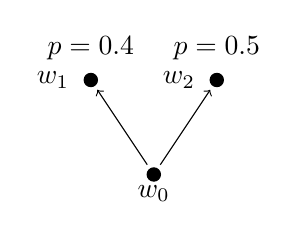
\begin{tikzpicture}[scale=0.8]
      % WORLDS  
      % w0
      \draw[fill] (0,-0.5) circle (3pt)
      +(0,-0)   node (w0)  {}  % used to label the circle 
      +(0,-0.3) node  {$w_0$}
      ;
            
      % w1
      \draw[fill] (-1,1) circle (3pt)
      +(0,0)   node (w1)  {}  % used to label the circle 
      +(-0.6,0) node{$w_1$}
      +(0,0.5) node{$p=0.4$}
      ;
      
      % w2
      \draw[fill] (1,1) circle (3pt)
      +(0,0)   node (w2)  {}  % used to label the circle 
      +(-0.6,0) node{$w_2$}
      +(0,0.5) node{$p=0.5$}
      ;
            
      % ARROWS
      \draw[->] (w0) -- (w1);
      \draw[->] (w0) -- (w2);
    \end{tikzpicture}
  \end{minipage}
  \begin{minipage}{0.5\linewidth}
    \[\small
    \begin{array}{l}
      % -----------------------------------------      
      \fcolorbox{black}{gray!10}{
        \begin{minipage}{16em}\small
          $W=\{\,w_0,\,w_1,\,w_2\,\}$
          \\
          $R =\{\,(w_0,w_1),\,(w_0,w_2)\,\}$
          \\
          $e(w_1,p) = 0.4,\,e(w_2,p) = 0.5$  
        \end{minipage}
      } % end box    
      % -----------------------------------------  
    \end{array}
    \]
  \end{minipage}
  \caption{The \GWCM-model  $\M^\ast=\stru{W,R,e}$.}
  \label{fig:ind}
\end{figure}
  


\subsection{Proofs}\label{app:proofs}

To prove Lemma~\ref{lemma:soundRule} we need the following definitions:
\begin{itemize}
\item Let $\M=\stru{W,R,e}$ be a $\GWM$-model, $w\in W$, $p\in\PV$ and
  $r\in[0,1]$, we denote with $e[(w,p):=r]$ the evaluation function
  $e'$ such that: $e'(w,p)=r$ and $e'(x,q)=e(x,q)$ for every pair
  $(x,q)\in W\times\PV$ such that $(x,q)\neq(w,p)$.

\item Let $\Ical$ be an $\M$-interpretation, let $w$ be a label of
  $\LC$ and $w^\star$ a world of $\M$.  By $\reass{\Ical}{w}{w^\star}$
  we denote the $\M$-interpretation $\Ical'$ such that $\Ical'(w) =
  w^\star$ and $\Ical'(x)= \Ical(x)$ for every $x\in \LC$ such that $x
  \neq w$.
\end{itemize}


\begin{lemmaref}{\ref{lemma:soundRule}}
  Let $\rho$ be an application of a rule of the calculus $\Calcw$, let
  $\Gamma$ be the conclusion of $\rho$ and let $\M$ be a \GWM-model.
  If $\M\models\G$, then there exists a premise $\G'$ of $\rho$ such
  that $\M\models\G'$.
\end{lemmaref}

\begin{proof}
  Let $\G$ be the conclusion of rule $\rho$ and let us assume
  $\M\models_\Ical\G$, where $\M=\stru{W,R,e}$; we show that there
  exist a premise $\G'$ of $\rho$, a $\GWM$-model
  $\M'=\stru{W',R',e'}$ and an $\M'$-interpretation $\Ical'$ such that
  $\M'\models_{\Ical'}\G'$.

  %%We denote $e[(w,p):=r]$, the assignment where $w\in\W'$, $p$ is a propositional variable
  %%and $r\in[0,1]_Q$
  
  The case $\rho=\ruleAxat$ has already been discussed in the paper.
  If $\rho$ is one of the rules $\land\lt$, $\land\gt$, $\lor\lt$,
  $\lor\gt$, $\ruleToLTAt$, $\ruleToLEQAt$, $\ruleToGAt$, the
  assertion easily follows.

  \smallskip

  Let $\rho$ be an application of $\to <$, where $\b\not\in \Vcal\cup{\bot}$:
  \[\small
  %% IMP LTS 
  \AXC{$\overbrace{w :\a > w : q,\,  w :\b \leq w :q,\,  w : q  < t,\,  \G_0}^{\G_1}$}    
  % ------------------------------------------    
  \RightLabel{$\to <$}
  \UIC{$\underbrace{w: \a\to \b < t,\,\G_0}_{\G}$}
  \DP
  \]
  By the hypothesis, it holds that $\M\models_{\Ical} w: \a\to \b < t$
  and $\M\models_{\Ical} \G_0$.  This implies that $e(\Ical(w), \a\to
  \b) < \Ical(t) \leq 1$, hence $e(\Ical(w),\a) > e(\Ical(w),\b)$ and
  $e(\Ical(w),\a\to \b) = e(\Ical(w),\b)$, thus $\M\models_\Ical w:\b
  < t$. Note that $q$ is a fresh propositional variable. Now let
  $r=e(\Ical(w),\b)$ and $\M'=\stru{W,R,e'}$ be the model where
  $e'=e[(\Ical(w),q):=r]$.  We remark that, for every constraint $\chi$
  not containing $q$, $\M\models_\Ical \chi$ iff $\M'\models_{\Ical}
  \chi$.  Since $\M\models_{\Ical} \G_0$ and $q$ does not occur in
  $\G_0$, we get $\M'\models_{\Ical} \G_0$.  It is easy to check that
  $\M'\models_{\Ical} w :\b \leq w:q$ and $\M'\models_{\Ical} w :\a >
  w:q$ and $\M'\models_{\Ical} w:q < t$, hence $\M'\models_{\Ical}
  \G_1$.

  \smallskip
  
  Let $\rho$ be an application of $\to \leq$, where $\b\not\in \Vcal\cup{\bot}$:
  \[
  %% IMP LTE 
  \AXC{$\overbrace{t \geq 1,\, \G_0}^{\G_1}$}    
  \AXC{$\overbrace{w :\a > w:q,\, w :\b \leq w:q,\, w:q \leq  t,\,\G_0}^{\G_2}$}    
  % ------------------------------------------    
  \RightLabel{$\to\leq$}
  \BIC{$\underbrace{w: \a\to \b \leq t,\,\G_0}_{\G}$}
  \DP
  \]
  By the hypothesis, $\M\models_{\Ical} w: \a\to \b \leq t$ and
  $\M\models_{\Ical} \G_0$, hence $e(\Ical(w), \a\to \b)\leq
  \Ical(t)$.  If $e(\Ical(w),\a) \leq e(\Ical(w),\b)$, then,
  $e(\Ical(w),\a\to \b) = 1$, which implies $1\leq \Ical(t)$, namely
  $\Ical(t) =1$.  It follows that $\M\models_\Ical t \geq 1$, hence
  $\M\models_\Ical \G_1$. Otherwise, $e(\Ical(w),\a) >
  e(\Ical(w),\b)$ and  $e(\Ical(w),\a\to \b) = e(\Ical(w),\b)$,
  hence $\M\models_\Ical w:\b \leq t$.  Note that $q$ is a fresh
  propositional variable.  Now let $r=e(\Ical(w),\b)$ and
  $\M'=\stru{W,R,e'}$ be the model where $e'=e[(\Ical(w),q):=r]$.  Since
  $\M\models_{\Ical} \G_0$ and $q$ does not occur in $\G_0$, we get
  $\M'\models_{\Ical} \G_0$.  Moreover, one can easily check that
  $\M'\models_{\Ical} w :\b \leq w:q$ and $\M'\models_{\Ical} w :\a >
  w:q$ and $\M'\models_{\Ical} w:q \leq t$; we conclude
  $\M'\models_{\Ical} \G_2$.

  \smallskip

  Let $\rho$ be an application of $\to \gt$, where $\b\not\in
  \Vcal\cup{\bot}$:
  \[
  %% IMP GT 
  \AXC{$\overbrace{w :\a \leq w:q,\,  w :\b \geq w:q,\,1\gt t,\, \G_0}^{\G_1}$}    
  \AXC{$\overbrace{w:\b \gt t,\, \G_0}^{\G_2}$}
  % ------------------------------------------       
  \RightLabel{$\to\gt$}
  \BIC{$\underbrace{w: \a\to \b \gt t,\,\G_0}_{\G}$}
  \DP
  \]
  By the hypothesis, $\M\models_{\Ical} w: \a\to \b \gt t$ and
  $\M\models_{\Ical} \G_0$, hence $e(\Ical(w),\a\to\b) \gt\Ical(t)$.
  We can reason as in the cases concerning rules $\to<$ and $\to\leq$.
  If $e(\Ical(w),\a) > e(\Ical(w),\b)$, then $e(\Ical(w),\a\to \b) =
  e(\Ical(w),\b)$, hence $\M\models_\Ical \G_2$.  Let us assume
  $e(\Ical(w),\a) \leq e(\Ical(w),\b)$.  In this case
  $e(\Ical(w),\a\to \b) = 1$, which implies $1 \gt \Ical(t)$.  Now let
  $r=e(\Ical(w),\a)$ and $\M'=\stru{W,R,e'}$ be the model where
  $e'=e[(\Ical(w),q):=r]$.  We can prove that $\M'\models_{\Ical} \G_1$.

  Let $\rho$ be an application of $\Box\lt$:
  \[
  \AXC{$\overbrace{R(w,w_1)\to w_1:\a \lt t,\,\Phibd{\G,w,w_1},\,\G_0}^{\G_1}$}
  % -----------------------------------------
  \RightLabel{$\Box\lt$}
  \UIC{$\underbrace{w:\Box\a \lt t,\,\G_0}_{\G}$}    
  \DP
  \]
  By the hypothesis, $\M\models_{\Ical} w:\Box\a \lt t$ and
  $\M\models_{\Ical} \G_0$, hence $e(\Ical(w),\Box \a)\lt
  \Ical(t)$. 
  % We have two cases.  If the world $\Ical(w)$ has no
  % $R$-successors, then $e(\Ical(w),\Box\a)=1$ and $t=1$ and
  % $\lt=\leq$. Since $\Ical(R(w,w_1))=0$ we have:
  % \begin{itemize}
  % \item $e(\Ical(w),R(w,w_1)\to w_1:\a)=1$;
  % \item $e(\Ical(w),\psi_1=R(w,w_1)\to w_1:\d)=1$ for every constraint of the
  %   kind $\psi_1\geq t$ in $\Phibd{\G,w,w_1}$;
  % \item $e(\Ical(w),\psi_2=R(w,w_1)\wedge w_1:\d)=0$ for every
  %   constraint of the kind $\psi_2\leq t$ in $\Phibd{\G,w,w_1}$.
  % \end{itemize}
  % Hence we get that $\M\models_{\Ical} \G_1$.  Otherwise if $\Ical(w)$
  % has at least one $R$-successor, 
  Since $\M$ is a $\GWM$-model, there exists a world $w^\star$ of $\M$
  such that $R(\Ical(w),w^\star)\to e(w^\star,\a)=e(\Ical(w),\Box\a)$.
  Let $\Ical'=\reass{\Ical}{w_1}{w^\star}$.  We remark that, for every
  constraint $\chi$ not containing $w_1$, $\M\models_\Ical \chi$ iff
  $\M\models_{\Ical'} \chi$. Since $w_1$ is a fresh world label, it
  does not occur in $\G_0$, and hence
  $\M\models_{\Ical'}\G_0$. Moreover:
  \begin{itemize}
  \item Since $e(\Ical(w),\Box \a)\lt \Ical(t)$ and $e(\Ical(w),\Box
    \a) = R(\Ical(w),w^\star)\to e(w^\star,\a)$, we have
    $R(\Ical(w),w^\star)\to e(w^\star,\a)\lt \Ical(t)$, and this
    implies $\M\models_{\Ical'} R(w,w_1)\to w_1:\a\lt t$.
    
  \item For every $\chi=R(w,w_1)\to w_1 : \d \gt
    t'\in\Phibd{\G,w,w_1}$, we have $w : \Box \b \gt t'\in \G_0$,
    hence $e(\Ical(w),\Box \b) \gt \Ical(t')$.  %%Since $\Ical(w) R w^\star$, 
    It follows that $R(\Ical(w),w^\star)\to e(w^\star,\b)\gt
    \Ical(t')$, and this implies $\M\models_{\Ical'} \chi$.

  \item For every $\chi=R(w,w_1)\wedge w_1 : \b \lt
    t'\in\Phibd{\G,w,w_1}$, we have $w : \Diam \b \lt t'\in \G_0$,
    hence $e(\Ical(w),\Diam \b) \lt
    \Ical(t')$. %% Since $\Ical(w) R w^\star$,
    It follows that $R(\Ical(w),w^\star)\land
    e(w^\star,\b)\lt\Ical(t')$, and this implies $\M\models_{\Ical'}
    \chi$.
  \end{itemize}
  We conclude $\M\models_{\Ical'} \G_1$. The case where $\rho$ is rule
  $\Diam\gt$ is similar.

  \smallskip
  
  Let $\rho$ be an application of $R\to <$:
  \[
  \AXC{$\overbrace{w':\a<R(w,w'),\,  w':\a  < t,\,  \G_0}^{\G_1}$}    
  % ------------------------------------------    
  \RightLabel{$R\to <$}
  \UIC{$\underbrace{R(w,w') \to w':\a < t,\,\G_0}_{\G}$}
  \DP
  \]
  By the hypothesis, it holds that $\M\models_{\Ical} R(w,w')\to w':
  \a < t$ and $\M\models_{\Ical} \G_0$.  This implies that
  $\Ical(R(w,w')\to w':\a) < \Ical(t) \leq 1$, hence
  $R(\Ical(w),\Ical(w')) > e(\Ical(w'),\a)$ and $\Ical(R(w,w')\to
  w':\a)= e(\Ical(w'),\a)$, thus $\M\models_\Ical w':\a < t$ and
  $\M\models_{\Ical} \G_1$.  The cases of the rules $R\land\gt$,
  $R\land\lt$, $R\to\leq$ and $R\to\gt$ are similar.
\end{proof}
  
  
\begin{lemma}\label{lemma:rulesDec}
  Let $\rho$ be an instance of a rule of the calculus $\Calcw$, let
  $\Gamma$ be the conclusion of $\rho$ and  $\G'$ any of the premises of $\rho$.
  Then,  $\G'\precc \G$.
\end{lemma}

  
\begin{proof}
  We only discuss two representative cases.
  Let us consider the following application of rule $\to < $:
  \[
  \begin{array}{l}
    \AXC{$\overbrace{w :\a > w : q,\,  w :\b \leq w :q,\,  w : q  < t,\,\D_w,\,\Theta}^{\G_1}$}    
    % ------------------------------------------    
    \RightLabel{$\to < $}
    \UIC{$\underbrace{w: \a\to \b < t,\,\D_w,\,\Theta}_\G$}
    \DP
    \\[2ex]
    \mbox{all the constraints in $\Delta_w$ have label $w$, no constraint in $\Theta$ has label $w$}
    \\[1ex]
    \G[w] =\{w:\a\to \b < t\} \cup \D_w 
    \hspace{3em}
    \G_1[w] =\{\,  w :\a > w : q,\,  w :\b \leq w :q,\,  w : q  < t  \,\}\cup\D_w
  \end{array}
  \]
  We have ($\cup$ denotes the multiset union):
  \[
  \sizem{\G} \,=\, \{\, \wg{\G[w]} \,\}\cup \sizem{\Theta}
  \hspace{3em}
  \sizem{\G_1} \;=\;
  \{\, \wg{\G_1[w]} \,\}    \cup \sizem{\Theta}    
  \]
  We prove that $\sizem{\G_1}\precm \sizem{\G}$. The following holds:
  \[
  \begin{array}{rcl}
    \wg{\G[w]}&\,=\, &\wg{w:\a\to \b < t} + \wg{\D_w} \;=\; \wg{\a} +  \wg{\b} + 1 +  \wg{\D_w} 
    \\[1ex]
    \wg{\G[w']}&\,=\, & \wg{w :\a > w : q} +\wg{w :\b \leq w :q} + \wg{w : q  < t } + \wg{\D_w}
    \\
    &\,=\,&  \wg{\a} +  \wg{\b} + 0 +  \wg{\D_w} 
  \end{array}
  \]
  Since $\wg{\G[w']} <  \wg{\G[w]}$, we get
  $\sizem{\G_1}\precm \sizem{\G}$, hence
  $\G_1\precc \G$.
  
  % -------------------------------------------------------------------------
  \smallskip
  Let us consider the following  application of $\Box\lt$:
  \[
  \begin{array}{l}
    \AXC{$\overbrace{\D_{w_1}, \;\D_w,\;\Theta}^{\G_1}$}
    % -----------------------------------------
    \RightLabel{$\Box\lt$}
    \UIC{$\underbrace{w:\Box\a \lt t,\;\Delta_w,\;\Theta}_\G$}    
    \DP
    \qquad \D_{w_1}\;=\;\{\,  R(w,w_1)\to w_1:\a \lt t\,\}\cup \Phibd{\Delta_w,w,w_1}
    \\[8ex]
    \mbox{all the constraints in $\Delta_w$ have label $w$, no constraint in $\Theta$ has label $w$}
    \\[1ex]
    \G[w] =\{w:\Box\a \lt t\} \cup \D_w
    \hspace{4em}
    \G_1[w] =\D_w
    \hspace{4em}
    \G_1[w_1]=\D_{w_1}
  \end{array}
  \]
  We have:
  \[
  \sizem{\G} \;=\; \{\, \wg{\G[w]} \,\}\cup \sizem{\Theta} 
  \hspace{4em}
  \sizem{\G_1} \;=\;
  \{\, \wg{\G_1[w]},\,   \wg{\G_1[w_1]} \,\}    \cup \sizem{\Theta}    
  \]  
  We prove that $\sizem{\G_1}\precm   \sizem{\G}$. To this aim,  we show that:
  
  \begin{enumerate}[label=(\roman*), ref=(\roman*),leftmargin=*]    
  \item\label{lemma:rulesDec:box1}
    $\wg{\G_1[w]} < \wg{\G[w]}$.
    
  \item\label{lemma:rulesDec:box2}
    $\wg{\G_1[w_1]} < \wg{\G[w]}$.
  \end{enumerate}
  The proof of point~\ref{lemma:rulesDec:box1} is immediate since $\G[w] =  \{w:\Box\a \lt t\}\cup\G_1[w]$.
  We prove~\ref{lemma:rulesDec:box2}. We have:
  \[
  \begin{array}{l}
    \wg{\G[w]}\;=\; \wg{w:\Box\a \lt t } + \wg{\Delta_w} \;=\; \wg{\a} + 2 +  \wg{\Delta_w}
    \\[1ex]
    \wg{\G_1[w_1]}\;=\; 
    \wg{ R(w,w_1)\to w_1:\a } + \wg{ \Phibd{\Delta_w,w,w_1} }
    \;=\;  \wg{\a} + 1 + \wg{ \Phibd{\Delta_w,w,w_1}}
  \end{array}
  \]
  To conclude the proof of~\ref{lemma:rulesDec:box2},
  we show that:
  
  \begin{enumerate}[label=(\roman*), ref=(\roman*),leftmargin=*,start=3]    
  \item\label{lemma:rulesDec:box3}
    $\wg{ \Phibd{\Delta_w,w,w_1}} <  \wg{\Delta_w}$.
  \end{enumerate}
  Let $\chi_1\in   \Phibd{\Delta_w,w,w_1}$. There exists $\chi\in \Delta_w$ such that one of the two
  following conditions holds:
  \begin{enumerate}[label=(\alph*), ref=(\alph*),leftmargin=*]    
  \item\label{lemma:rulesDec:box3a}
    $\chi = w:\Box \b \gt t'$ and $\chi_1 = R(w,w_1)\to w_1 : \b \gt t'$;
    
  \item\label{lemma:rulesDec:box3b}
    $\chi = w:\Diam \b \lt t'$ and $\chi_1 = R(w,w_1)\land w_1 : \b \lt t'$.
  \end{enumerate}
  In both cases, it holds that $\wg{\chi_1}= \wg{\b} +1$ and
  $\wg{\chi}= \wg{\b} +2$, hence $\wg{\chi_1} < \wg{\chi}$; this
  proves~\ref{lemma:rulesDec:box3}.  From~\ref{lemma:rulesDec:box1}
  and~\ref{lemma:rulesDec:box2} it follows that $\sizem{\G_1}\precm
  \sizem{\G}$, hence $\G_1\precc \G$.
\end{proof}





%\begin{figure}
%  \centering
  
%  \includegraphics[angle=90, width=0.3\textwidth]{prova.png}
%\end{figure}




%%% Local Variables: 
%%% mode: latex
%%% TeX-master: "goedelModalLogicWitnessNonCrisp"
%%% End: 
